\documentclass[conference]{IEEEtran}
\usepackage{amsmath, amssymb, amsfonts}
\usepackage{xcolor}
\usepackage{tikz}

\begin{document}

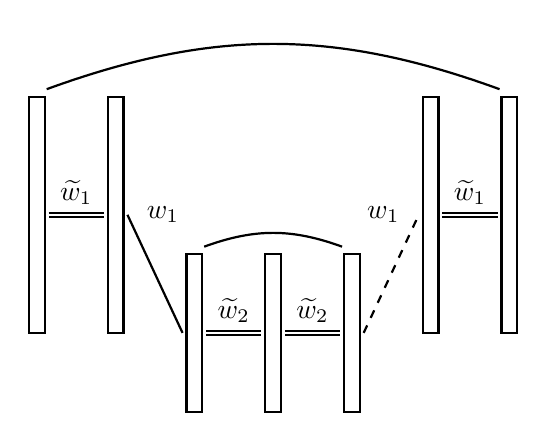
\begin{tikzpicture}
        \draw[black, thick] (0,-1.5) rectangle (0.2, 1.5);
        \node[] at (0.1, 1.55) (a1) {};
        \draw[thick, double] (0.25,0) -- (0.95, 0) node[above, midway] {$\widetilde{w}_1$};
        \draw[black, thick] (1.0,-1.5) rectangle (1.2, 1.5);
        \draw[thick] (1.25,0) -- (1.95, -1.5);
        \node[] at (1.7, 0) {$w_{1}$};
        \draw[black, thick] (2.0,-2.5) rectangle (2.2, -0.5);
        \node[] at (2.1, -0.45) (b1) {};
        \draw[thick, double] (2.25,-1.5) -- (2.95, -1.5) node[above, midway] {$\widetilde{w}_2$};
        \draw[black, thick] (3.0,-2.5) rectangle (3.2, -0.5);
        \draw[thick, double] (3.25,-1.5) -- (3.95, -1.5) node[above, midway] {$\widetilde{w}_2$};
        \draw[black, thick] (4.0,-2.5) rectangle (4.2, -0.5);
        \node[] at (4.1, -0.45) (b2) {};
        \draw[thick] (b1) to[out=20,in=160] (b2);
        \draw[thick, dashed] (4.25, -1.5) -- (4.95, 0);
        \node[] at (4.5, 0) {$w_{1}$};
        \draw[black, thick] (5.0,-1.5) rectangle (5.2, 1.5);
        \draw[thick, double] (5.25,0) -- (5.95, 0) node[above, midway] {$\widetilde{w}_1$};
        \draw[black, thick] (6.0,-1.5) rectangle (6.2, 1.5);
        \node[] at (6.1, 1.55) (a2) {};
        \draw[thick] (a1) to[out=20,in=160] (a2);
    \end{tikzpicture}

\end{document}